\subsection{Image Rectification}
Before an image can be used for calculation, some image processing had to be performed on the frames in order to get rid of the distortions and account for the camera's extrinsic parameters. 

\subsubsection{Frames of reference}
In order to get the right equations for the rectification of the images, some frames of reference that can be followed throughout the rest of the calculations were defined.

\begin{figure}[H]
    \centering
    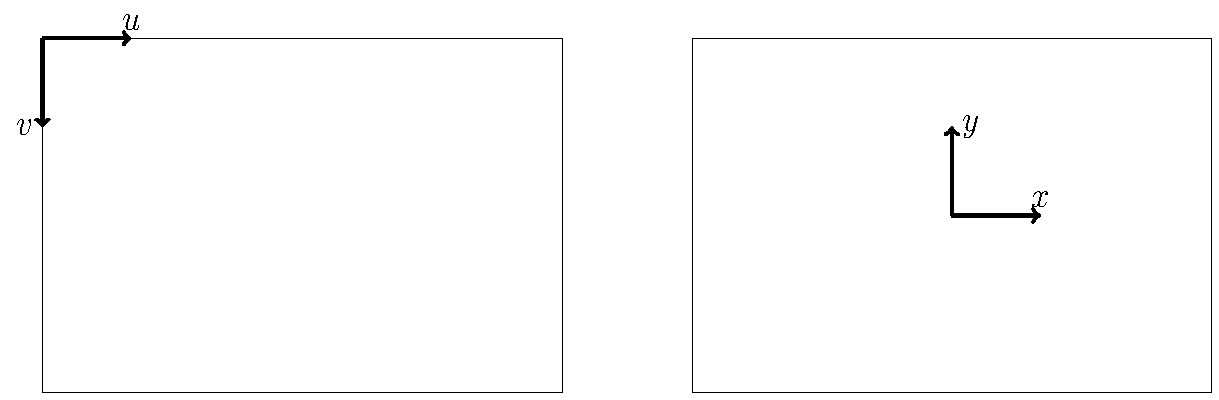
\includegraphics[width = \textwidth]{Figures/camera_coordinate_frame.pdf}
    \caption{Camera frame of reference}
    \label{fig:img_FOR}
\end{figure}

All frames read by the OpenCV library are images which follow the $uv$ frame of reference presented in Figure \ref{fig:img_FOR}. In order to apply the extrinsic parameters (which is explained in a later section) on certain points of the image, a frame of reference conversion is required. Extrinsic parameters and the transformation from 2D to 3D are applied on an $xy$ frame of reference similar to the one presented in Figure \ref{fig:img_FOR}. Once in 3D, the points will be expressed in the $XYZ$ frame of reference presented in Figure \ref{fig:vehicle_FOR}.

\begin{figure}[H]
    \centering
    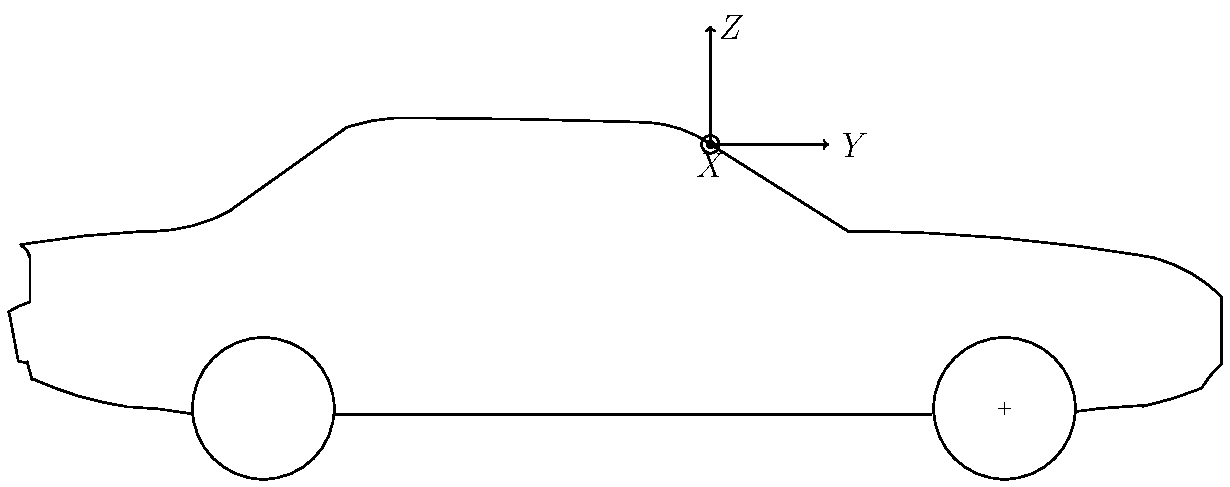
\includegraphics[width = 0.8\textwidth]{Figures/V_FBD.pdf}
    \caption{Vehicle frame of reference}
    \label{fig:vehicle_FOR}
\end{figure}



\subsubsection{Intrinsic Parameters}
The intrinsic parameters in this project are limited to the radial and tangential distortions which are explained in the literature review and in \cite{wang2008new}. For rectifying an image using the OpenCV library, the camera matrix and an array of distortion coefficients are required as an input. The camera matrix is defined by its focal lengths and the coordinates of its principal center which are provided from VTTI such that
\begin{equation}
    A = 
     \begin{bmatrix}
    f_u & 0 & c_x\\
    0 & f_v & c_y\\
    0 & 0 & 1
    \end{bmatrix}
\end{equation}
where
\begin{equation}
    f = 
     \begin{bmatrix}
    f_u \\ f_v
    \end{bmatrix}
    =
    \begin{bmatrix}
    347.1960 \\ 352.3415
    \end{bmatrix}
\end{equation}

\begin{equation}
    c = 
    \begin{bmatrix}
    c_x \\ c_y
    \end{bmatrix}
    =
    \begin{bmatrix}
    241.5788 \\ 188.9012
    \end{bmatrix}
\end{equation}
The array of distortion coefficients is expressed as

\begin{equation}
    DistortionCoefficients = 
    \begin{bmatrix}
    k_1 ~~ k_2 ~~ p_1 ~~ p_2 ~~ k_3
    \end{bmatrix}
\end{equation}
where $k_1,k_2 ~ and ~ k_3$ are radial distortion coefficients, and $p_1~and~p_2$ are tangential distortion coefficients. Those coefficients are acquired from VTTI. The array used for the rectification is hence

\begin{equation}
    DistortionCoefficients = 
    \begin{bmatrix}
    -0.432387 ~~ 0.183867 ~~ -0.038207 ~~ 0.000657 ~~ 0.000187 
    \end{bmatrix}
\end{equation}

It is important to keep in mind that not all videos in the database are recorded using the same camera. This means that using those distortion coefficients for all the videos is one of the assumptions in the project.


\subsubsection{Extrinsic Parameters}
\label{sec:meth_ExtrensicParameters}

Any point $(x',y')$ in the $xy$ image frame can be rectified with the extrinsic parameters to a point $(x,y)$ which can be used for further processing and distance calculation later on. This can be seen in Figure \ref{fig:homo_rect} where point $p$ has the coordinates $(x,y)$ after the rectification is applied to point $p'$. 
\begin{figure}[H]
    \centering
    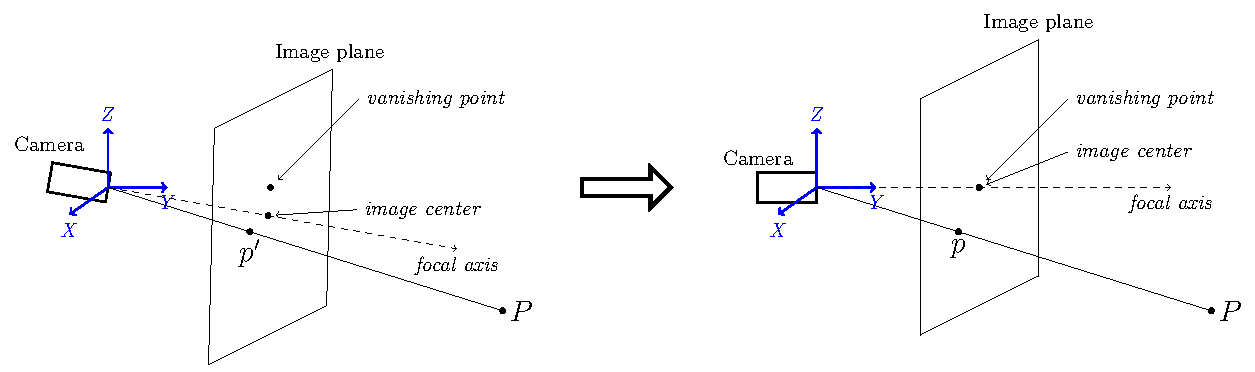
\includegraphics[width = \textwidth]{Figures/homo_rectify.pdf}
    \caption{Rectifying the camera's extrinsic parameters with homography}
    \label{fig:homo_rect}
\end{figure}

This rectification is interpreted as a transformation matrix called the homography matrix $\bf{H}$. The homography matrix is in general a relation between two images of the same object taken from a different camera or pose. In this case, the different camera poses are of the same dashcam before and after accounting for the extrinsic parameters which are the pitch and yaw of the SV. The theory of this transformation matrix is described here. A point $(x',y')$ is transformed to $(x,y)$ using the homography matrix $\bf{H}$.

\begin{equation}
    \begin{bmatrix}
    lx\\ly\\l
    \end{bmatrix}
    = \bf{H}
    \begin{bmatrix}
    x' \\ y' \\ 1
    \end{bmatrix}
    = 
    \begin{bmatrix}
    r_{11} & r_{12} & f_u r_{13}\\
    r_{21} & r_{22} & f_v r_{23}\\
    \frac{r_{31}}{f_u} & \frac{r_{32}}{f_v} & r_{33}
    \end{bmatrix}
    \begin{bmatrix}
    x' \\ y' \\ 1
    \end{bmatrix}
\end{equation}
where the $l$ is an arbitrary scaling factor and the components $r_{i,j}$ form the \textit{Euler-Rodrigues rotation matrix} \cite{DAI2015144} which states
\begin{equation}
    {\bf R} = {\bf I} + \left( sin \alpha \right) {\bf J_v} + \left( 1 - cos \alpha \right) {\bf J_v^2} = r(i,j)
\end{equation}
where we will define $\alpha = \begin{Vmatrix} \Omega \end{Vmatrix}$,  $\Omega = (\theta, \phi, \psi)$, $\textbf{v} = (v_x,v_y,v_z) = \frac{\Omega}{\alpha}$, and \textbf{$J_v$} is a skew-symmetric matrix defined as
\begin{equation}
\bf{J_v} = 
\begin{pmatrix}
0 & -v_z & v_y \\
v_z & 0 & -v_x \\
-v_y & v_x & 0
\end{pmatrix}    
\end{equation}

\begin{equation}
{\bf R} \approx {\bf I} + 
\begin{bmatrix}
0 & \phi & -\psi \\
-\phi & 0 & \theta \\
\psi & -\theta & 0
\end{bmatrix} =
\begin{bmatrix}
1 & \phi & -\psi \\
-\phi & 1 & \theta \\
\psi & -\theta & 1
\end{bmatrix}    
\end{equation}
Here, the angles $\theta, ~ \psi ~ and ~ \phi$ are the camera's pitch, yaw and roll angles respectively. So the homography matrix becomes

\begin{equation}
\bf{H} = 
\begin{bmatrix}
1 & \phi & -f_u \psi \\
-\phi & 1 & f_v \theta \\
\frac{\psi}{f_u} & -\frac{\theta}{f_v} & 1
\end{bmatrix}     
\end{equation}

In this project, it is assumed that the roll angle $\phi$ of the vehicle is negligible. Since the camera and the SV are assumed to share the same angels, the homography matrix narrows down to

\begin{equation}
\bf{H} = 
\begin{bmatrix}
1 & 0 & -f_u \psi \\
0 & 1 & f_v \theta \\
\frac{\psi}{f_u} & -\frac{\theta}{f_v} & 1
\end{bmatrix}   
\end{equation}

In order to get the pitch and yaw angles ($\theta$ and $\psi$), the vanishing point method will be used. In an image plane, all lines lying on one plane and parallel to each other will meet at a point called the vanishing point. Considering the ground plane, this means that parallel lane lines will intersect at a certain vanishing point in the image plane. In 3D, this point has a coordinate $Y=\infty$, meaning it is on the horizon. Joining all parallel lines of different slopes together will eventually create a set of vanishing points which, if joined, make up the horizon (also referred to as vanishing line) \cite{WANG2004}.

Finding the vanishing point in the image plane is a straight forward task. Whether it is by automatic lane detection, or by manually selecting points on the lane lines, an equation of each lane line can be developed. The vanishing point is then the intersection of those two lines. Considering two points on each lane, where points $(x_{11},y_{11})$ and $(x_{12},y_{12})$ are on one line, and $(x_{21},y_{21})$ and $(x_{22},y_{22})$ are on the other, the coordinates of the vanishing point become:
\begin{align}
    x_{vp} &= \frac{b_2-b_1}{m_1-m_2},\\
    y_{vp} &= m_1 x_{vp} + b_1
\end{align}
where each line has an equation $y = mx + b$, $m$ is the slope of the lane line and $b$ is the y-intercept.
% Show a figure.

Now from the location of the vanishing point in relation to the centre of the image, the pitch and yaw can be estimated, and the homography matrix can be created that for the vanishing point $vp$ as follows:
\begin{align}
    0 &= x_{vp} + f_u \psi\\
    0 &= y_{vp} + f_v \theta
\end{align}
This can be assumed since the mapping of the vanishing point using $\bf{H}$ should give a zero vector. Hence, the pitch and yaw angles are calculated as:
\begin{align}
    \psi &= \frac{-x_{vp}}{f_u}\\
    \theta &= \frac{-y_{vp}}{f_v}
\end{align}